\documentclass{beamer}
\usetheme{CambridgeUS}
\usefonttheme{serif}
\usepackage[sfmath]{kpfonts}

\title{TCC}
\author{Thales A. de O. Barretto}
\date{7 Dez. 2022}

% ####################################################
% Referências ABNT
% ####################################################
\usepackage[%
    alf,
    abnt-emphasize=bf,
    bibjustif,
    recuo=0cm,
    abnt-url-package=url,       % Utiliza o pacote url
    abnt-refinfo=yes,           % Utiliza o estilo bibliográfico abnt-refinfo
    abnt-etal-cite=3,
    abnt-etal-list=3,
    abnt-thesis-year=final
]{abntex2cite}                  % Configura as citações bibliográficas conforme a norma ABNT

% ####################################################
% Pacotes
% ####################################################
\usepackage[utf8]{inputenc}                                 % Codificação do documento
\usepackage[T1]{fontenc}                                    % Seleção de código de fonte
\usepackage{booktabs}                                       % Réguas horizontais em tabelas
\usepackage{color, colortbl}                                % Controle das cores
\usepackage{float}                                          % Necessário para tabelas/figuras em ambiente multi-colunas
\usepackage{graphicx}                                       % Inclusão de gráficos e figuras
\usepackage{icomma}                                         % Uso de vírgulas em expressões matemáticas
\usepackage{indentfirst}                                    % Indenta o primeiro parágrafo de cada seção
\usepackage{microtype}                                      % Melhora a justificação do documento
\usepackage{multirow, array}                                % Permite tabelas com múltiplas linhas e colunas
\usepackage{subeqnarray}                                    % Permite subnumeração de equações
\usepackage{lastpage}                                       % Para encontrar última página do documento
\usepackage{verbatim}                                       % Permite apresentar texto tal como escrito no documento, ainda que sejam comandos Latex
\usepackage{amsfonts, amssymb, amsmath}                     % Fontes e símbolos matemáticos
\usepackage[algoruled, portuguese]{algorithm2e}             % Permite escrever algoritmos em português
%\usepackage[scaled]{helvet}                                % Usa a fonte Helvetica
\usepackage{times}                                          % Usa a fonte Times
%\usepackage{palatino}                                      % Usa a fonte Palatino
%\usepackage{lmodern}                                       % Usa a fonte Latin Modern
\usepackage[bottom]{footmisc}                               % Mantém as notas de rodapé sempre na mesma posição
\usepackage{ae, aecompl}                                    % Fontes de alta qualidade
\usepackage{latexsym}                                       % Símbolos matemáticos
\usepackage{lscape}                                         % Permite páginas em modo "paisagem"
\usepackage{picinpar}                                      % Dispor imagens em parágrafos
\usepackage{scalefnt}                                      % Permite redimensionar tamanho da fonte
\usepackage{subfig}                                        % Posicionamento de figuras
\usepackage{upgreek}                                       % Fonte letras gregas

% ####################################################
% Fonte similar a Arial (Helvetica)
% ####################################################
\renewcommand*\familydefault{\sfdefault}

\definecolor{verde}{rgb}{0,0.5,0}
\usepackage{listings}
\lstset{
  language=C,
  basicstyle=\ttfamily\small,
  keywordstyle=\color{blue},
  stringstyle=\color{verde},
  commentstyle=\color{red},
  extendedchars=true,
  showspaces=false,
  showstringspaces=false,
  numbers=left,
  numberstyle=\tiny,
  breaklines=true,
  backgroundcolor=\color{white},
  breakautoindent=true,
  captionpos=b,
  xleftmargin=0pt,
}

\usepackage{pdfpages}

% -----------------------------------------------------------------------------
% Configurações do PDF Final
\makeatletter
\hypersetup{
    portuguese,
    colorlinks=true,   % true: "links" coloridos; false: "links" em caixas de texto
    linkcolor=blue,    % Define cor dos "links" internos
    citecolor=blue,    % Define cor dos "links" para as referências bibliográficas
    filecolor=blue,    % Define cor dos "links" para arquivos
    urlcolor=blue,     % Define a cor dos "hiperlinks"
    breaklinks=true,
    pdftitle={\@title},
    pdfauthor={\@author},
    pdfkeywords={abnt, latex, abntex, abntex2}
}
\makeatother

% -----------------------------------------------------------------------------
% Altera o aspecto da cor azul
\definecolor{blue}{RGB}{41,5,195}

% -----------------------------------------------------------------------------
% Redefinição dos Labels
\renewcommand{\algorithmautorefname}{Algoritmo}
\def\equationautorefname~#1\null{Equa\c c\~ao~(#1)\null}

% -----------------------------------------------------------------------------
% Cria um indice remissimo
\makeindex

% -----------------------------------------------------------------------------
% Hifenização de palavras que nào estão no discionário
\hyphenation{
    qua-dros-cha-ve
    Kat-sa-gge-los
}


\begin{document}
\begin{frame}\label{capa}
\begin{centering}
    {\scriptsize 
    \textbf{FACULDADE DE TECNOLOGIA DE CATANDUVA\\
    }}
    \vfill

    {\normalsize
    Aplicação de sensor Inercial de baixo custo em sistemas robóticos autônomos:
    captura de atitude e movimento de um robô móvel com 
    o sensor MPU-6050 em Raspberry Pi\\
    }
    \vspace{16pt}

    {\tiny
    Trabalho de Graduação para o curso de Tecnologia em Automação Industrial\\
    }
    \vfill

    {\normalsize
    {\textbf{Thales Antunes de Oliveira Barretto}}\\
    \vspace{16pt}
    {\scriptsize Orientador: Prof.~MSc.~Tácio Luiz de Souza Barbeiro}\\
    }
\end{centering}
\end{frame}

\begin{frame}{Apresentação}
    Nossa apresentação será dividida em:
    \begin{itemize}
        \item Justificativa, Objetivos
        \item Métodos e materiais
        \item Resultados e conclusão
    \end{itemize}
\end{frame}

\begin{frame}{Justificativa}
        Sistemas robóticos, em geral, são empregados quando a intervenção humana revela-se muito onerosa, perigosa ou ineficaz. A capacidade de operar de forma autônoma, nestes casos, é uma característica valiosa. Sensores de medição inercial podem ser úteis nos sistemas de controle robóticos.
\end{frame}

\begin{frame}{Objetivos}

    Nosso principal objetivo consiste em avaliar a utilidade do sensor inercial modelo MPU-6050 em sistemas robóticos autônomos.\\
    \vfill

    Estabelecemos como metas:
    \begin{itemize}
    \item criar driver para o sensor ligado a uma \emph{Raspberry Pi}.
    \item criar aplicação para capturar de dados de movimento.
    \item simular a captura de dados de um robô autônomo.
    \end{itemize}

\end{frame}

\begin{frame}{Materiais:Sensor MPU-6050}

    MPU-6050 é um sensor de medição inercial ('IMU') com sete instrumentos: três acelerômetros três giroscópios e um sensor de temperatura. A interface de comunicação principal obedece o padrão ``I2C''.

    \begin{figure}[H]
        \centering
        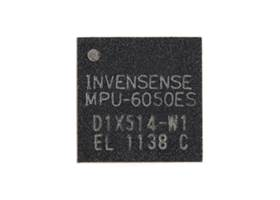
\includegraphics[width=0.5\textwidth]{figuras/mpu6050-sensor-top-straight.jpg}
    \end{figure}

\end{frame}


\begin{frame}{Materiais:Sensor MPU-6050}

    A orientação dos sensores em relação ao encapsulamento obedece a regra da mão direita:

    \begin{figure}[H]
        \centering
        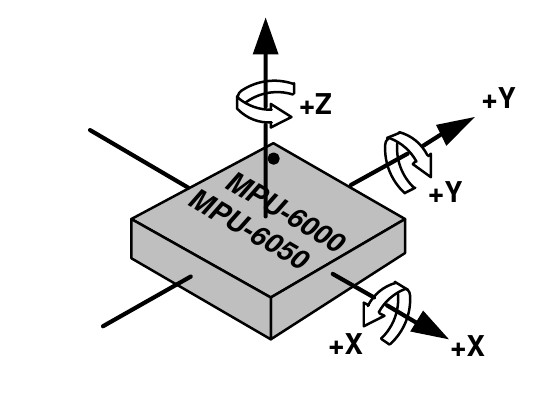
\includegraphics[width=0.5\textwidth]{figuras/mpu6050-diagram-axis.jpg}
    \end{figure}

\end{frame}

\begin{frame}{Materiais:Sensor MPU-6050}

    Comercialmente disponível já montado em placa módulo:

    \begin{figure}[H]
        \centering
        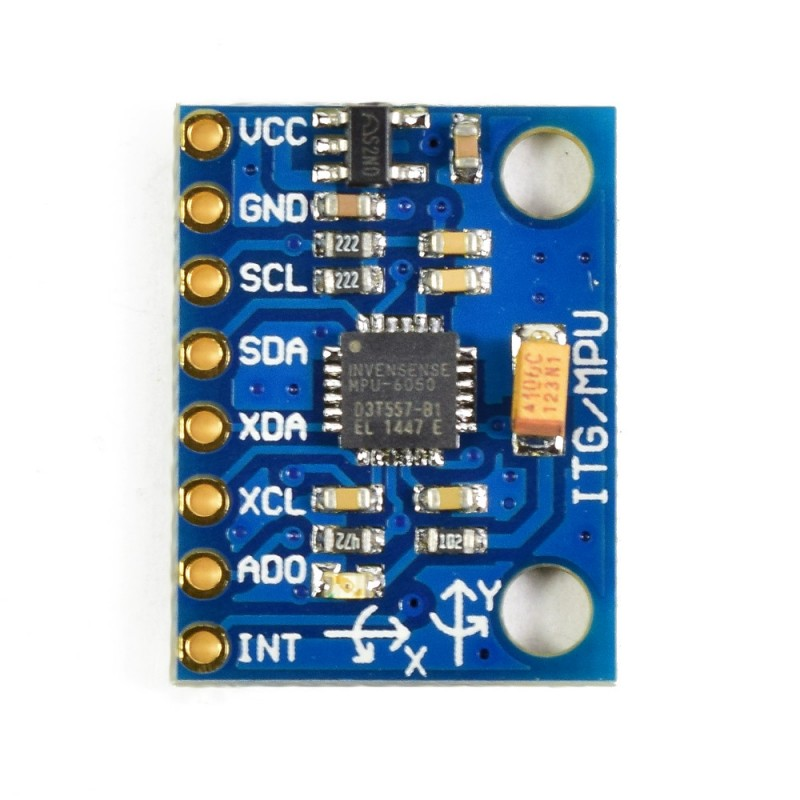
\includegraphics[width=0.5\textwidth]{figuras/mpu6050-board-top.jpg}
    \end{figure}

\end{frame}

\begin{frame}{Materiais:Raspberry Pi}

    O sensor foi anexado a um computador Raspberry Pi para desenvolvimento:
    \begin{figure}[H]
        \centering
        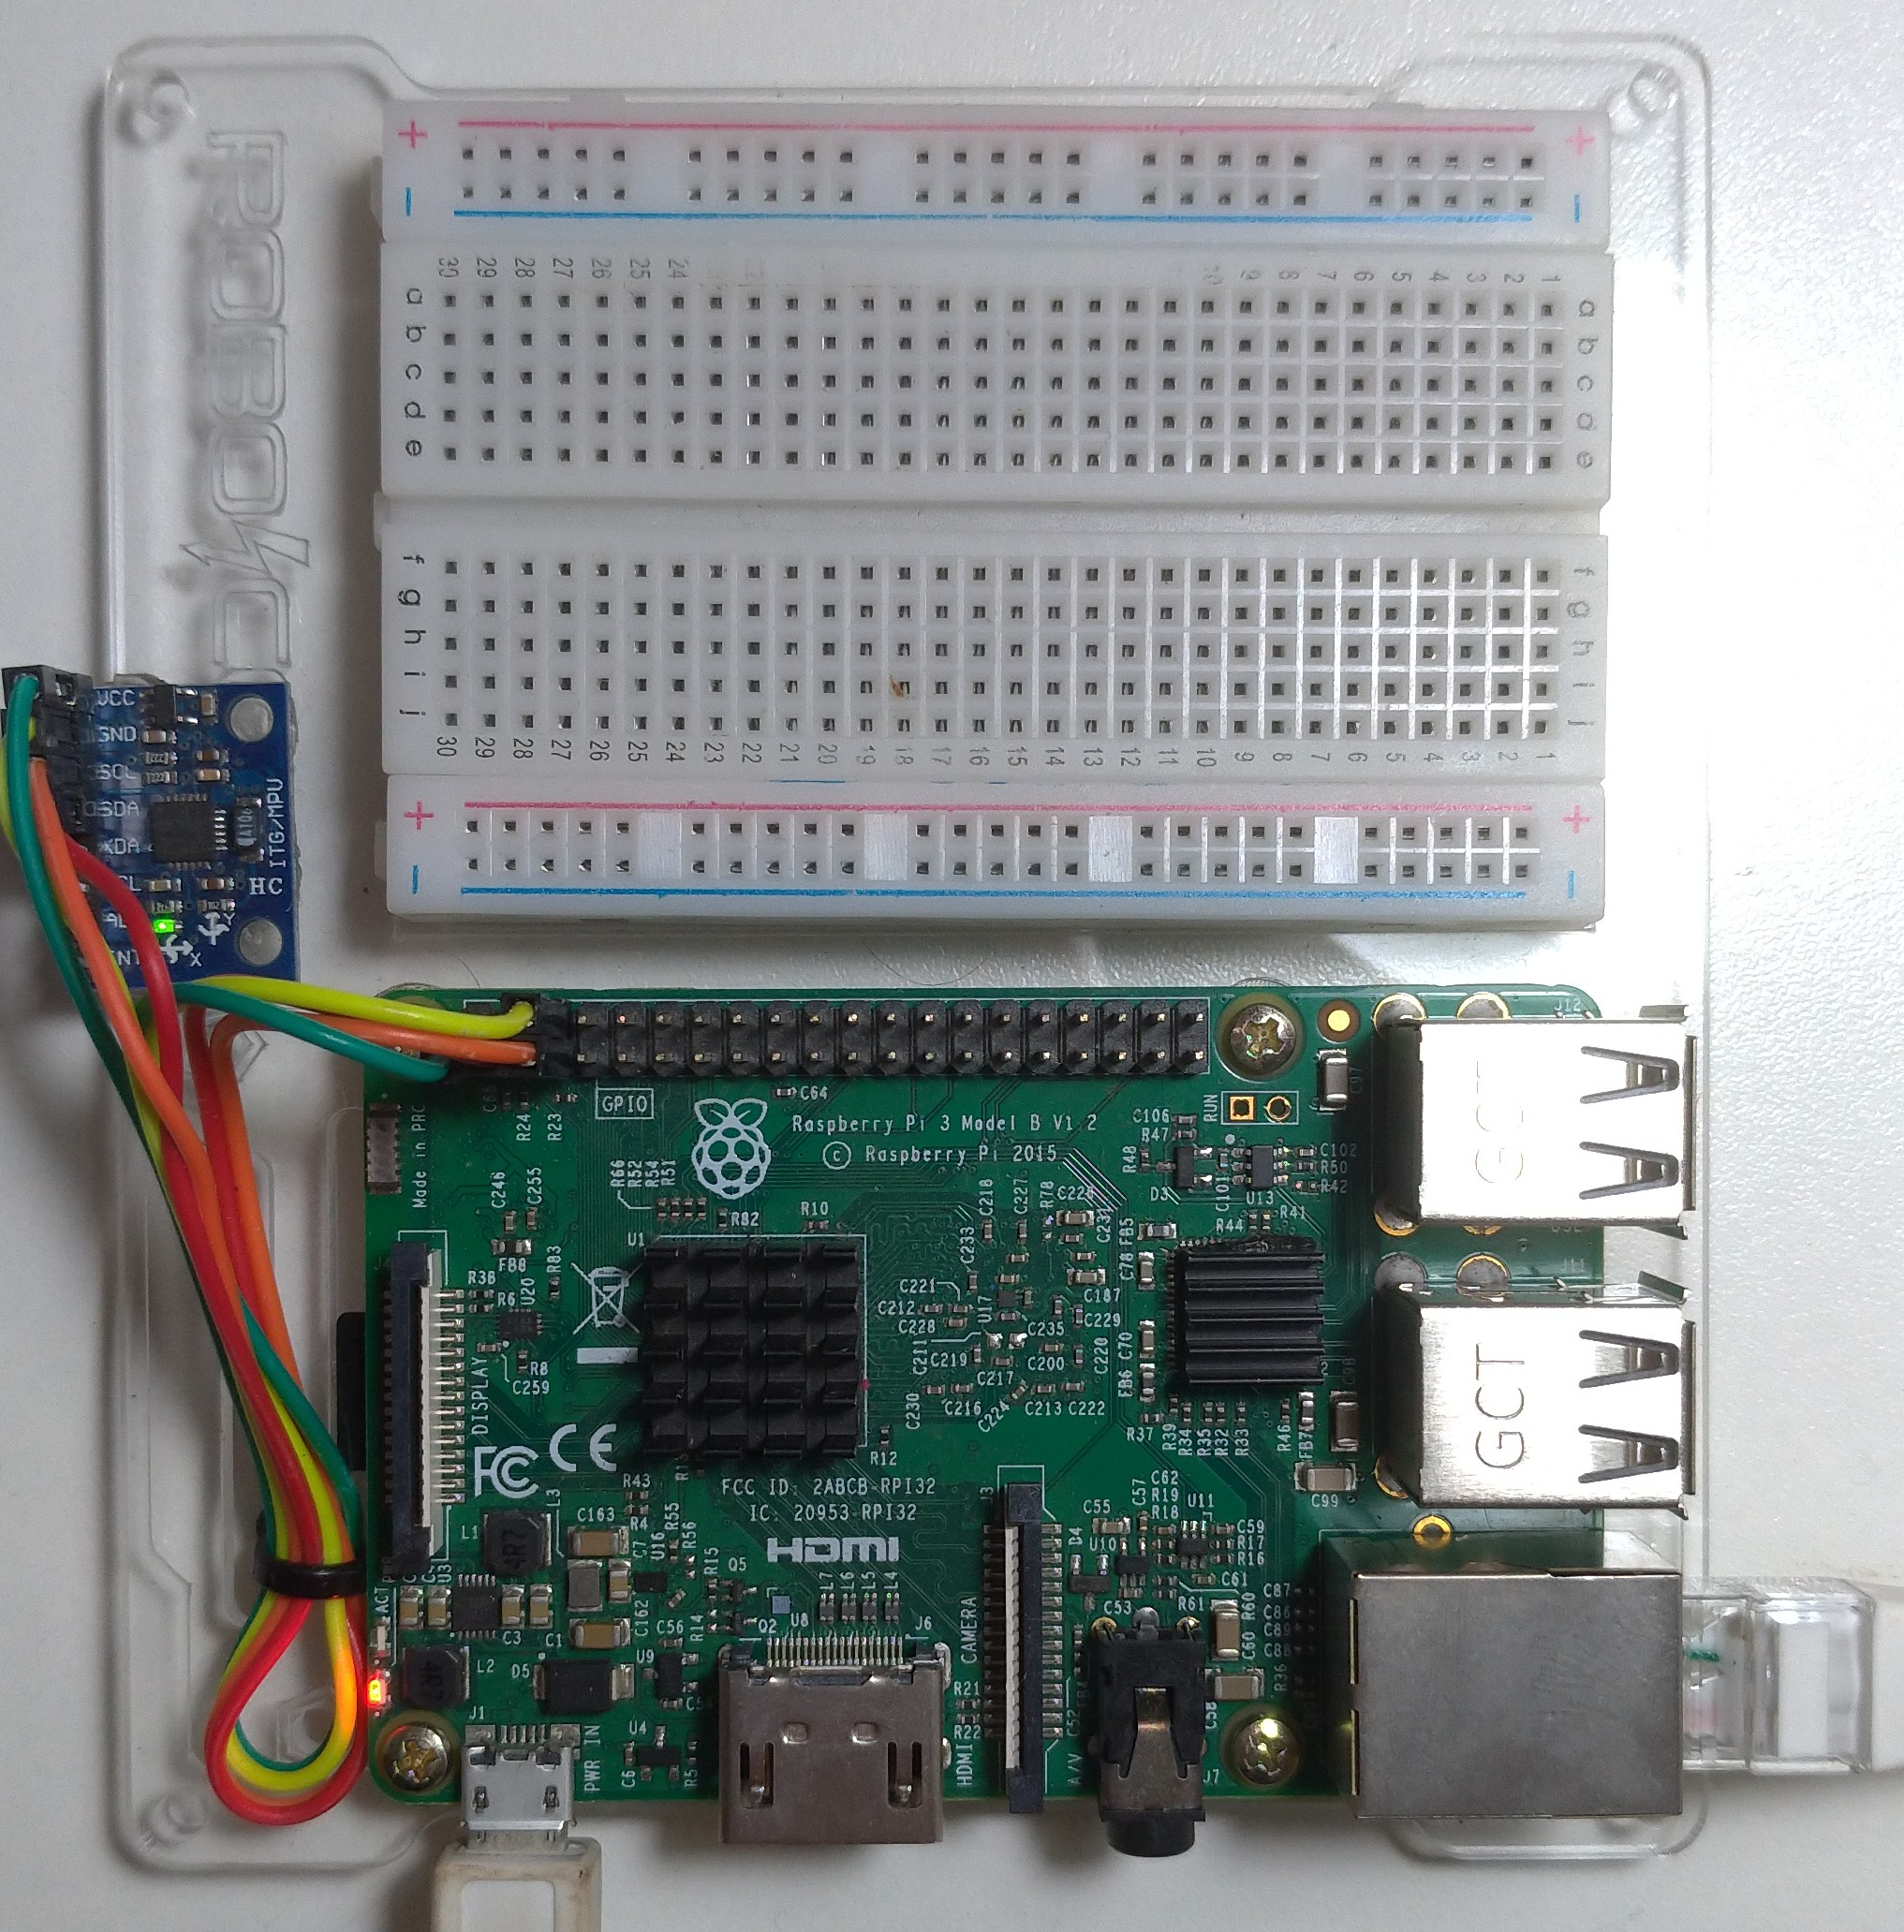
\includegraphics[width=0.5\textwidth]{figuras/mpu6050-proto-top.jpg}
    \end{figure}

\end{frame}

\begin{frame}{Métodos: Atitude e ângulos de Euler}

    Descrevemos a atitude de um corpo em ângulos de Euler na sequência \emph{``yaw, pitch, roll''} (guinada, arfada e rolagem), de rotações anti-horárias (regra da mão direita), levando do sistema (\(ned\)) - ``North-East-Down'' (Norte, Leste, Abaixo) ao sistema (\(frd\)) - ``Front-Right-Down'' (Avante, Direita, Abaixo), fixo no robô:

\begin{enumerate}
    \item Rotação anti-horária sobre eixo \(z\), ou \(\psi\) positivo (\textit{``compass heading''})
    \item Rotação anti-horária sobre novo eixo \(y'\), ou \(\theta\) positivo (\textit{pitch})
    \item Rotação anti-horária sobre novo eixo \(x''\), ou \(\phi\) positivo (\textit{roll})
\end{enumerate}

\end{frame}

\begin{frame}{Métodos: Atitude e matrizes de rotação}

Matrizes de rotação:

\begin{align*}
    C_{f\!r\!d\!/\!n\!e\!d} &=
    \begin{bmatrix}
        1               &  0            &  0             \\
        0               &  \cos{\phi}   &  \sin{\phi}    \\
        0               & -\sin{\phi}   &  \cos{\phi}
    \end{bmatrix}
    \begin{bmatrix}
        \cos{ \theta}   &  0            & -\sin{\theta} \\
        0               &  1            &  0            \\
        \sin{ \theta}   &  0            &  \cos{\theta}
    \end{bmatrix}
    \begin{bmatrix}
        \cos{\psi}      &  \sin{\psi}   &  0             \\
       -\sin{\psi}      &  \cos{\psi}   &  0             \\
        0               &  0            &  1
    \end{bmatrix} \\
    C_{f\!r\!d\!/\!n\!e\!d} &=
    \begin{bmatrix}
        c\theta c\psi   & c\theta s\psi & -s\theta    \\
        \left(-c\phi s\psi + s\phi s\theta c\psi \right)
        &  \left( c\phi c\psi + s\phi s\theta s\psi \right)
        &  s\phi c\theta                                 \\
        \left( s\phi s\psi + c\phi s\theta c\psi \right)
        &  \left( -s\phi c\psi + c\phi s\theta s\psi \right)
        & c\phi c\theta
    \end{bmatrix}
\end{align*}

Intervalo de validade:
\begin{align*}
    -\pi  < \phi \leq \pi \\
    -\frac{\pi}{2} \leq \theta \leq \frac{\pi}{2} \\
    -\pi < \psi \leq \pi
\end{align*}
\end{frame}

\begin{frame}{Métodos: Atitude e derivada de um vetor}

Genericamente a derivada de um vetor é similar à de um escalar:
\begin{equation*}
    \frac{\mathrm{d}}{\mathrm{d}t} \mathbf{p}_{A/B} =  \lim_{\delta t \rightarrow 0 } \begin{bmatrix}
        \displaystyle\frac{\mathbf{p}_{A/B} (t + \delta t) - \mathbf{p}_{A/B} (t) }{\delta t}
    \end{bmatrix}
\end{equation*}

Um vetor pode apontar em qualquer direção por meio de rotação:
\begin{figure}[h]
    \centering
    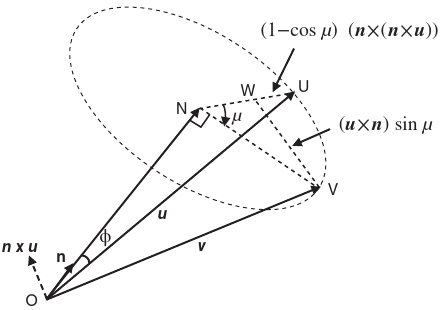
\includegraphics[width=0.5\textwidth, keepaspectratio]{figuras/figure1.2-1.png}\label{fig1.2-1}
\end{figure}

\end{frame}


\begin{frame}{Métodos: Atitude e velocidade angular}

Na figura acima obtemos \(\mathbf{v}\):
    \begin{align}
        \mathbf{v} &= \mathbf{u} + \left(1 - {\cos{\mu}}\right) \left(\mathbf{n}\!\times\!\left(\mathbf{n}\!\times\!\mathbf{u}\right)\right) - \left(\mathbf{n}\!\times\!\mathbf{u}\right){\sin{\mu}}\label{eq:rotation-formula-a} %\tag{1.2-5a}
    \end{align}
    \begin{align}
        \mathbf{v} = \left(1 - {\cos{\mu}}\right) \mathbf{n}\!\left(\mathbf{n}\cdot\mathbf{u}\right) + \mathbf{u}{\cos{\mu}} - \left(\mathbf{n}\!\times\!\mathbf{u}\right){\sin{\mu}} \label{eq:rotation-formula-b}  % \tag{1.2-5b}
    \end{align}

    Para \(\delta\mu \ll 1 \text{rad}\), definindo \(\mathbf{v} = \mathbf{u} + \delta \mathbf{u}\), e aplicamos (\ref{eq:rotation-formula-a}) obtendo:
\begin{equation*}
    \delta \mathbf{u} \approx -\!\sin(-\delta\mu)\mathbf{n}\!\times\!\mathbf{u} \approx (\mathbf{n}\!\times\!\mathbf{u})\delta\mu
\end{equation*}

Dividindo por \(\delta t\), no limite onde \(\delta t \rightarrow 0\), definimos \(\mathbf{\omega} \equiv \dot{\mu}\mathbf{n}\) obtendo:

\begin{equation}
    \dot{\mathbf{u}} = \mathbf{\omega}\!\times\!\mathbf{u}\label{eq:vector-derivative} %\tag{1.4-1}
\end{equation}

Este vetor \(\mathbf{\omega}\) denominamos \textit{vetor velocidade angular} que associamos sistema de coordenadas fixado no corpo.

\end{frame}

\begin{frame}{Métodos: Atitude, ângulos de Euler e velocidade angular}
Relação taxas de ângulos de Euler e velocidade angular:

\begin{align*}
    \mathbf{\omega}^{frd}_{b/r} &= \begin{bmatrix} \dot\phi \\ 0 \\0 \end{bmatrix}
    + C_{\phi} \begin{pmatrix}
        \begin{bmatrix} 0 \\ \dot\theta \\ 0 \end{bmatrix}
        + C_{\theta}\begin{bmatrix} 0 \\ 0 \\ \dot\psi \end{bmatrix}
    \end{pmatrix} \\
    \mathbf{\omega}^{frd}_{b/r} 
    &\equiv \begin{bmatrix} P \\ Q \\ R \end{bmatrix}
    = \begin{bmatrix}
        1 & 0 & -\sin{\theta} \\
        0 & \cos{\phi} & \sin{\phi}\cos{\theta} \\
        0 & -\sin{\phi} & \cos{\phi}\cos{\theta}
    \end{bmatrix}
    \begin{bmatrix}
        \dot\phi \\
        \dot\theta \\
        \dot\psi
    \end{bmatrix}
\end{align*}

\ldots sendo \(P\), \(Q\), \(R\), os componentes do vetor velocidade angular do corpo expressos no sistema \(frd\), respectivamente, rolagem (\emph{``roll''}), arfada (\emph{``pitch''}) e guinada (\emph{``yaw''}).

\end{frame}

\begin{frame}{Métodos: Atitude e mudança de atitude}

 A transformação inversa é dada por:

\begin{align*}\label{eq:1.4-4}% \tag{1.4-4}
    \begin{bmatrix}
        \dot\phi \\
        \dot\theta \\
        \dot\psi
    \end{bmatrix}
    =
    \begin{bmatrix}
        1 & \sin{\phi}\tan{\theta} & \cos{\phi}\tan{\theta} \\
        0 & \cos{\phi} & -\sin{\phi} \\
        0 & \frac{\sin{\phi}}{\cos{\theta}} & \frac{\cos{\phi}}{\cos{\theta}}
    \end{bmatrix}
    \begin{bmatrix}
        P \\ Q \\ R
    \end{bmatrix}
\end{align*}

Para simplificar, definimos \(\mathbf{\Phi} \equiv \left[\phi \theta \psi \right]^T \) e reescrevemos:

\begin{equation}\label{eq:1.4-5}% \tag{1.4-5}
    \dot{\mathbf{\Phi}} = H \left( \mathbf{\Phi} \right) \mathbf{\omega}^{frd}_{b/r}
\end{equation}

\end{frame}

\begin{frame}{Métodos: Equações do movimento e rotação}
Derivadando um vetor em relação em sistemas móveis obteremos \(^{a}\dot{\mathbf{p}}\):

\begin{figure}[H]
    \centering
    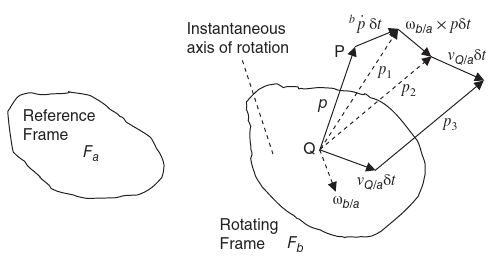
\includegraphics[width=0.5\textwidth, keepaspectratio]{figuras/figure1.4-1.png}\label{fig1.4-1}
\end{figure}

Desse modo, no instante \(\delta t\), \(\mathbf{p}_{2} \!-\! \mathbf{p}\) temos:
\begin{equation*}
    \mathbf{p}_{2} - \mathbf{p} = {^{b}\dot{\mathbf{p}}} \delta t + \left( \mathbf{\omega}_{b/a} \! \times \!\mathbf{p} \right) \delta t
\end{equation*}

Dividindo por \(\delta t\) no limite em que \(\delta t \rightarrow 0\) resulta na equação\footnotemark{}:
\begin{equation} \label{eq:1.4-2}
    {^{a}\dot{\mathbf{p}}} = {^{b}\dot{\mathbf{p}}} + {\mathbf{\omega}_{b/a} \! \times \!\mathbf{p}}
\end{equation}
\end{frame}

\begin{frame}{Métodos: Equações do movimento em quadros móveis}

Generalizando para sistemas móveis:

\begin{figure}[H]
    \centering
    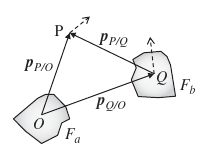
\includegraphics[width=0.25\textwidth, keepaspectratio]{figuras/figure1.5-1.png}\label{fig1.5-1}
\end{figure}

\begin{equation*}
    \mathbf{v}_{P/a} = \mathbf{v}_{P/b} + \left( \mathbf{v}_{Q/a} + \mathbf{\omega}_{b/a}\!\times\!\mathbf{p}_{P/Q} \right),
\end{equation*}
\begin{equation*}
    \mathbf{a}_{P/a} = \mathbf{a}_{P/b} + \overbrace{\mathbf{a}_{Q/a} + {{\mathbf{\alpha}_{b/a}}\!\times\!{\mathbf{p}_{P/Q}}} + \underbrace{{{\mathbf{\omega}_{b/a}}\!\times\!{\left({\mathbf{\omega}_{b/a}}\!\times\!{\mathbf{p}_{P/Q}}\right)}}}_{\text{aceleração centrípeta}}}^{\text{aceleração de transporte}} + \underbrace{{2\mathbf{\omega}_{b/a}\!\times\!\mathbf{v}_{P/b}}}_{\text{aceleração de Coriolis}} \label{eq:1.5-4}
\end{equation*}

\end{frame}

\begin{frame}{Métodos: Equações do movimento e simplificações}

Para um sensor fixo no quadro \(F_{b}\) do robô então \(\mathbf{a}_{P/b}\) desaparece:
\begin{equation*}
    {\mathbf{a}_{P/a}} = {\mathbf{a}_{Q/a}} + {\mathbf{\alpha}_{b/a}}\!\times\!{\mathbf{p}_{P/Q}} + {\mathbf{\omega}_{b/a}}\!\times\!\left({\mathbf{\omega}_{b/a}}\!\times\!{\mathbf{p}_{P/Q}}\right)
\end{equation*}

Sejam \(F_{i}\)  e  \(F_{e}\) quadros inercial e fixo na Terra, com \(Q\) e \(O\) coincidentes no centro de massa da Terra, então o \(\mathbf{p}_{P/Q}\) é um vetor posição geocêntrico, e \(\mathbf{a}_{Q/a}=0\). Considerando a rotação da Terra constante, então a derivada de \(\mathbf{\omega}_{b/a}\) também desaparece e chegamos em:
\begin{equation} \label{eq:1.5-5}
    {\mathbf{a}_{P/i}} = {\mathbf{a}_{P/e}} + {\mathbf{\omega}_{e/i}}\!\times\!\left({\mathbf{\omega}_{e/i}}\!\times\!{\mathbf{p}_{P/O}}\right) + 2\mathbf{\omega}_{e/i}\!\times\!\mathbf{v}_{P/e}
\end{equation}
\end{frame}

\begin{frame}{Métodos: Equações do movimento e Forças}

Aplicando a segunda lei de Newton e reescrevendo em termos de forças:
\begin{equation*}
    \text{Força aparente} = \text{força verdadeira} - \underbrace{m \left[{\mathbf{\omega}_{e/i}}\!\times\!\left({\mathbf{\omega}_{e/i}}\!\times\!{\mathbf{p}_{P/O}}\right)\right]}_{\text{força centrífuga}} - \underbrace{m \left( 2{\mathbf{\omega}_{e/i}}\!\times\!{\mathbf{v}_{P/e}}\right)}_{\text{força de Coriolis}}
\end{equation*}

Força verdadeira (\(F\)) é a soma das \textit{forças de contato}. A força do \textit{campo gravitacional da Terra} corresponde a \(m\mathbf{G}\). O vetor gravidade da Terra (\(g\)) é dado por \(\mathbf{g}~=~\mathbf{G}~-~\text{aceleração centrípeta}\): 
\begin{equation*}\label{eq:1.5-6}
    \mathbf{a}_{P/e} = \frac{F}{m} + g - {2 \mathbf{\omega}_{e/i}}\!\times\!{\mathbf{v}_{P/e}}
\end{equation*}

Para baixas velocidades podemos desconsiderar a aceleração de Coriolis:
\begin{equation*}
    \mathbf{a}_{P/e} = \frac{F}{m} + g
\end{equation*}


\end{frame}

\begin{frame}{Métodos: Equações do movimento e acelerômetros}

Um acelerômetro mede, indiretamente a força \(\mathbf{F}\) que equilibra uma \emph{massa de prova} com o encapsulamento. Com o campo gravitacional atuando na massa de prova \(m\), seja \(\mathbf{F}/m\) a força por unidade de massa aplicada à massa de prova, chamada de força específica, \(\mathbf{f}\) determinamos a aceleração \(\mathbf{a}\) da massa de prova:
\begin{equation*}
    \mathbf{a} = \dfrac{\mathbf{F}}{m} + \mathbf{G} \equiv \mathbf{f} + \mathbf{G}.
\end{equation*}

Quando um acelerômetro, com vetor de posição geocêntrico\footnotemark{} \(\mathbf{p}\), está estacionário em relação à Terra, temos a leitura de aceleração:
\begin{align}
    \mathbf{f} &= \mathbf{a} - \mathbf{G} = -\!{\mathbf{g}} \label{eq:1.6-29}
\end{align}
\end{frame}

\begin{frame}{Métodos: Equações do movimento e acelerômetros}
Para um acelerômetro com três eixos ortogonais \(x\), \(y\) e \(z\), situado num ponto \({P}\) fixado no quadro \({F}_{frd}\) do corpo de um robô, com vetor de posição geocêntrico \(\mathbf{p}\), designamos \(\mathbf{G}_{p}\) o vetor projeção da força nos elementos sensores, \(\mathbf{g}\) o vetor aceleração da gravidade expresso em múltiplos da \emph{gravidade padrão}, \(\mathbf{a}\) a aceleração do corpo tomada no quadro de referência da Terra, e \({C}_{frd/ned}\) a matriz de rotação do quado \(frd\) em relação ao \(ned\), obtendo a equação:
\begin{equation*}
    {\mathbf{G}}_p = \begin{bmatrix} {G}_{px} \\ {G}_{py} \\ {G}_{pz} \end{bmatrix} = {C}_{frd/ned}\left(\mathbf{g} - {\mathbf{a}}\right)
\end{equation*}
\end{frame}

\begin{frame}{Métodos: Equações do movimento e acelerômetros}

Quando (\(\mathbf{a}\approxeq0\)) podemos obter:
\begin{align*}
    {\mathbf{G}}_p &=
    \begin{bmatrix} 
    -\sin{\theta}\\
    \cos{\theta}\sin{\phi}\\
    \cos{\theta}\cos{\phi}
    \end{bmatrix} \\
{\phi}_{xyz} &= \tan^{-1}\left(\frac{G_{py}}{G_{pz}}\right) \\
{\theta}_{xyz} &= \tan^{-1}\left(\frac{-G_{px}}{\sqrt{{{G_{py}}^{2}}+{{{G}_{pz}}^2}}}\right) \\
    &-\pi  < \phi \leq \pi \\
    &-\frac{\pi}{2} \leq \theta \leq \frac{\pi}{2} \\
\end{align*}
\end{frame}

\begin{frame}{Métodos: Equações do movimento em plano tangente}
    Aproximando as equações para um plano tangente à superfície da Terra:

\begin{align*}
    {^{b}{\dot{\mathbf{v}}_{cm/e}}} &= \textstyle{\frac{1}{m}} \mathbf{F} + \mathbf{g} - {\left( \mathbf{\omega}_{b/i} + \mathbf{\omega}_{e/i} \right)} \times \mathbf{v}_{cm/e}
\end{align*}

e, tomando a Terra por referencial inercial (\(\mathbf{\omega}_{e/i} \equiv 0 , \mathbf{\omega}_{b/i} \equiv \mathbf{\omega}_{b/e}\)):

\begin{align}\label{eq:1.7-16c}
   {^{b}{\dot{\mathbf{v}}_{cm/e}}} &= \textstyle{\frac{1}{m}} \mathbf{F} + \mathbf{g} - \mathbf{\omega}_{b/e} \times \mathbf{v}_{cm/e}
\end{align}

Para completar, o vetor \(\mathbf{g}\) em coordenadas do plano tangente será:

\begin{equation}
\mathbf{g}^{tp} = {\begin{bmatrix} 0 & 0& g_{D} \end{bmatrix}}^{T}
\end{equation}

\end{frame}

\begin{frame}{Métodos: Modelo cinemático}
Para os elementos das equações de estado, estabelecemos que
\begin{align*}
    &\mathbf{p}^{tp}_{cm/Q} \equiv \begin{bmatrix} p_{N} & p_{E} & p_{D} \end{bmatrix}^{T},&
    &\mathbf{\Phi} \equiv \begin{bmatrix} \phi & \theta & \psi \end{bmatrix}^{T} \\
    &\mathbf{v}^{frd}_{cm/e} \equiv \begin{bmatrix} U & V & W \end{bmatrix}^{T},&
    &{\dot{\mathbf{\Phi}}} \equiv \begin{bmatrix} \dot{\phi} & \dot{\theta} & \dot{\psi} \end{bmatrix}^{T} \\
    &{^{b}{\dot{\mathbf{v}}}^{frd}_{cm/e}} \equiv \begin{bmatrix} {\dot{U}} & {\dot{V}} & {\dot{W}} \end{bmatrix}^{T}, &
    &\mathbf{\omega}^{frd}_{b/e} \equiv \begin{bmatrix} P & Q & R \end{bmatrix}^{T}
\end{align*}
\end{frame}

\begin{frame}{Métodos: Equações de estado}

Para os nossos propósitos, o nosso vetor de estado fica assimm:
\begin{align*}
    {X}^{T} = \begin{bmatrix} {\left( \mathbf{p}^{tp}_{cm/O} \right)}^{T} & \mathbf{\Phi}^{T} \end{bmatrix}
\end{align*}

O vetor de entrada:
\begin{equation*}
    \mathbf{u}^{T} = \begin{bmatrix} \dot{U} & \dot{V} & \dot{W} & P & Q & R \end{bmatrix}^{T}
\end{equation*}

Derivando as variáveis de estado:
\begin{align*}
    C_{frd/tp} &= fn \left( \Phi \right) \\
    \dot{\Phi} &=  H \left( \Phi \right) {\mathbf{\omega}^{frd}_{b/e}} \\
    {^{e}{\dot{\mathbf{p}}^{tp}_{cm/Q}}} &= {C_{tp/frd}}{\mathbf{v}^{frd}_{cm/e}} \\
    {^{b}{\dot{\mathbf{v}}^{frd}_{cm/e}}} &= \textstyle{\frac{1}{m}} {\mathbf{F}^{frd}} + {C_{frd/tp}}{\mathbf{g}^{tp}} - {\tilde{\mathbf{\omega}}^{frd}_{b/e}} {\mathbf{v}^{frd}_{cm/e}}
\end{align*}

\end{frame}

\begin{frame}{Métodos: Equações de estado}

As equações cinemáticas para um plano tangente á Terra resultam em:
\begin{align*}
    &\dot{\phi}   =  P + \tan{\theta} \left( Q \sin{\phi} + R \cos{\phi} \right) \\
    &\dot{\theta} =  Q \cos{\phi} - R \sin{\phi} \\
    &\dot{\psi}   =  \left( Q \sin{\phi} + R \cos{\phi} \right) / \cos{\theta} \\
    &\dot{p_{N}}  =  U c \theta c \psi  + V ( -c \phi s \psi + s \phi s \theta c \psi ) + W ( s \phi s \psi + c \phi s \theta c \psi) \\
    &\dot{p_{E}}  =  U c \theta s \psi  + V (  c \phi s \psi + s \phi s \theta s \psi ) + W (-s \phi c \psi + c \phi s \theta c \psi) \\
    &\dot{h}      =  U s \theta - V s \phi c \theta - W c \phi c \theta
\end{align*}

Para obtermos uma solução no domínio do tempo e obter a trajetória do veículo só nos resta a solução numérica dessas equações.

\end{frame}

\begin{frame}{Métodos: Sinais e métodos numéricos}
A solução numérica da trajetória do estado exige que, dada uma condição inicial \(x\left(t_{0}\right)\) e o termo de entrada \(\mathbf{u}(t)\), calculamos o estado em intervalos de tempo constante \(t\) pequenos o bastante para considerar o termo \(\mathbf{u}\) constante entre \(kt\) e \(\left(k+1\right)t\) sem modificar significativamente os resultados:
\begin{align*}
    &x \left( t_{0} + kt \right), \quad k = 1,2 \ldots \\
    &\dot{x} \left( t \right) = f \big(x\left(t\right), \mathbf{u}\left(t\right)\big)\label{eq:3.4-1b}
\end{align*}
\end{frame}

\begin{frame}{Métodos: Método de Euler}
A questão acima, conhecida como \emph{problema do valor inicial}, será enfrentada aqui pelos métodos \emph{Runge-Kutta} (RK). Considere o problema do valor inicial na sua forma mais simples: uma equação diferencial autônoma de primeira ordem com uma condição de limite específica:
\begin{equation*}\label{eq:3.4-2}
    {\frac{\textrm{d}x}{\textrm{d}t}} = f \left( x, t \right), \quad
    x \left( t_{0} \right) = x_{0}
\end{equation*}

Podemos estabelecer uma relação entre o problema de encontrar valores determinados para~(\ref{eq:3.4-2}) e a série de Taylor:
\begin{equation*}\label{eq:3.4-3}
    x \left(t_{0} + T \right) = x \left(t_{0}\right) + T \dot{x}\left(t_{0}\right) + \frac{T^{2}}{2!} \ddot{x}\left(t_{0}\right) + \ldots
\end{equation*}

O método mais simples, pouco preciso e que exige um período \(T\) muito pequeno, consiste em truncar a série após a primeira derivada, conhecido por método de Euler ou de \emph{primeira ordem}:
\begin{equation*}\label{eq:3.4-4}
    x_{E}\left(t_{0} + T \right) \approx x \left( t_{0} \right) + T f\left(x\left(t_{0}\right), t_{0}\right)
\end{equation*}
\end{frame}

\begin{frame}{Métodos: Método trapezoidal}
O \emph{método trapezoidal}, por exemplo, ou de \emph{segunda ordem}, é um pouco mais preciso, e consiste em primeiro estimar a integral pelo método de Euler, então usar a média das derivadas no início e no fim do período para uma estivativa mais precisa. Pode ser expresso empregando índices \(E\) e \(T\) para os passos obtidos pelos métodos de \emph{Euler} e \emph{trapezoidal}:
\begin{align*}\label{eq:3.4-5}
    x_{E}\left(t + T\right) &= x\left(t\right) + T f\left(x\left(t\right),t\right) \\
    \dot{x}_{E}\left(t + T\right) &= {f{\left( x_{E} {\left( t + T \right)}, t+T \right)}} \\
    x_{T}\left(t + T\right) &= x\left(t\right) + \frac{T}{2} \left[ \dot{x}\left(t\right) + \dot{x}_{E}\left(t + T\right) \right],
\end{align*}
\end{frame}

\begin{frame}{Métodos: Sinais discretos}

    Para o processamento digital (em tempo discreto) assumimos a condição de  ``zero-order-data-hold'' (ZOH) em relação aos sinais amostrados, conforme ilustrado na figura:
\begin{figure}[H]
    \centering
    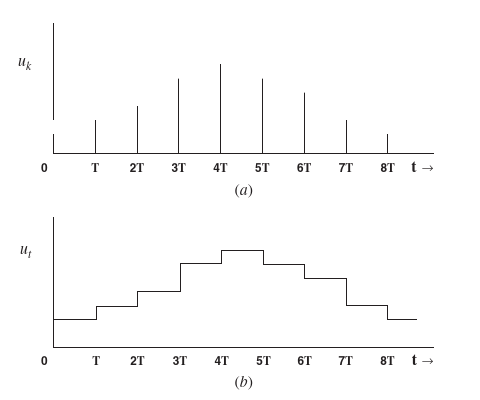
\includegraphics[width=0.5\textwidth, keepaspectratio]{figuras/figure7.2-2.png}\label{fig7.2-2}
\end{figure}

\end{frame}

\begin{frame}{Métodos: Driver}

    Oferece como abstrações ema estrutura de dados que representa o estado atual do sensor MPU-6050 e métodos para operar os dados e configurações. A nossa implementação impõe a captura simultânea de dados de todos os sensores, em intervalos regulares de tempo, mediante o uso de um buffer interno e configurações apropriadas.
    \vspace{12pt}
    Deve ser compilado e instalado como uma biblioteca, empregando a arquitetura ``driver in userspace'' das interfaces i2c/smbus do sistema Linux.
    \vspace{12pt}
    Código aberto a contribuições e licenciado sob a ``MIT License''.
    \vspace{12pt}
    Disponível em https://github.com/ThalesBarretto/libmpu6050.

\end{frame}

\begin{frame}{Métodos: Captura de movimento}

    Aplicação de console que implementa as equações de estado e métodos numéricos mencionados acima. Trabalha com a abstração de série de estados e integração numérica da trajetória do estado entre uma amostra e outra. Oferece um filtro complementar para estimativa da atitude bem como a integração pelo método trapezoidal da atitude e posição.
    \vspace{12pt}
    Código aberto a contribuições e licenciado sob a ``MIT License''.
    \vspace{12pt}
    Disponível em https://github.com/ThalesBarretto/mpu6050.

\end{frame}

\begin{frame}{Resultados}

Ao final do teste estacionário obtivemos estimativas de atitude \((\phi,\theta,\psi)\) e posição~\((p_{n},p_{e},p_{u})\) a seguir:

\begin{table}[ht]
    \centering
    \begin{tabular}{r r r r r r r}
        teste & \(\phi (^{o})\) & \(\theta(^{o})\) & \(\psi(^{o})\) & \(p_{n}(\textrm{m})\) & \(p_{e}(\textrm{m})\) & \(p_{u}(\textrm{m})\)  \\
        \toprule
        1 & +0.09 & +0.05 & +0.05 & -0.308 & -1.174 & +127.510  \\
        2 & +0.09 & -0.01 & -0.01 & +0.396 & -1.458 & +100.242  \\
        3 & +0.06 & -0.02 & -0.02 & -0.647 & -0.636 & +105.201  \\
        \bottomrule
    \end{tabular}
    \label{Tab:tabela1}
\end{table}
    
\end{frame}

\begin{frame}{Conclusão}

Os resultados apontam para a exploração de sensores melhores e métodos matemáticos e estatísticos mais sofisticados, por exemplo, o emprego de física na formulação de Hamilton para superar as limitações de validade quanto aos ângulos, integração por métodos de Runge-Kutta de quarta e quinta ordem para melhor estabilidade e precisão da integração numérica, fusão de dados com sensores magnéticos e de posição absoluta por filtro de Kalman, uso de inteligência artificial e aprendizado de máquina para correção dos dados, entre outros.

\end{frame}

\begin{frame}
\begin{centering}
    \normalsize
    {\textbf{Thales Antunes de Oliveira Barretto}}\\

    {\small{thales.barretto.git@gmail.com}}\\
\end{centering}
\end{frame}

\end{document}
